\documentclass[11pt,addpoints]{exam}

\usepackage{tikz}
\usetikzlibrary{calc, angles}
\usepackage{tkz-tab}
\usepackage[margin=1.5cm]{geometry}
\usepackage{amsmath}

\begin{document}

\begin{center}
    \Huge{Contrôle sur les suites}
\end{center}

\begin{questions}
\qformat{\textbf{Q\thequestion)}\hfill(\thepoints)}
\question[2]
\begin{parts}
    \part Compléter la suite de nombres suivante : 1 3 5 7 9 ? ? ?
    \part Comment passe-t-on d'un nombre au suivant ? 
    \part Comment appelle-t-on ce type de suite ?
\end{parts}
\question[2]
\begin{parts}
    \part Compléter la suite de nombres suivante : 3 6 12 24 ? ? ?
    \part Comment passe-t-on d'un nombre au suivant ?
    \part Comment appelle-t-on ce type de suite ?
\end{parts}
\question[3] Soit la suite $(u_n)$ définie par $u_n = 3n+7$. Calculer $u_0$, $u_5$, $u_{10}$.
\question[3] Soit la suite $(v_n)$ définie par $v_n = -2n+1$. Calculer $v_0, v_3, v_5$.
\question[1] Soit la suite $(w_n)$ définie par $w_0 = 3$ et $w_{n+1} = w_n - 4$. Calculer $w_1$ et $w_2$.


\question[3] Pour chacune des suites ci-dessous, dire si elle est croissante, décroissante ou ni l'un ni l'autre.

\newcommand{\point}[2]
{
    \draw ($(#1,#2) + (-0.1,-0.1)$) -- ($(#1,#2) + (0.1,0.1)$) ($(#1,#2) + (-0.1,0.1)$) -- ($(#1,#2) + (0.1,-0.1)$); 
}

\begin{center}
    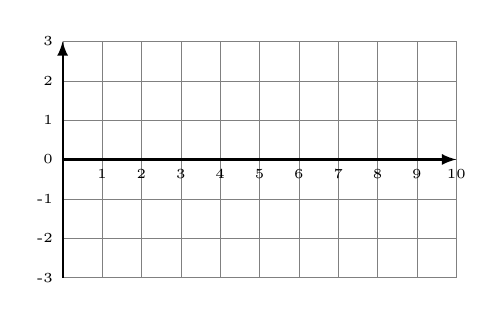
\begin{tikzpicture}[scale=0.5,domain=0:10]
        \draw[line width =0.03mm, gray] (0,-3) grid (10,3);
        \draw[thick, -latex] (0,0) -- (10,0);
        \draw[thick, -latex] (0,-3) -- (0,3);
        \foreach \x in {1,...,10} {
            \node[below] at (\x,0) {\tiny\x};
        }
        \foreach \y in {-3,-2,...,3} {
            \node[left] at (0,\y) {\tiny\y};
        }
        \foreach \n in {0,1,...,10} {
            \point{{\n}}{{sqrt(\n)-1}}
        }
    \end{tikzpicture}
    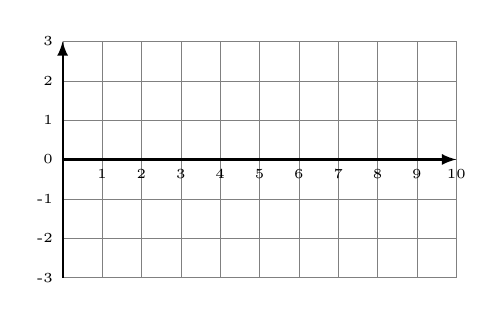
\begin{tikzpicture}[scale=0.5,domain=0:10]
        \draw[line width =0.03mm, gray] (0,-3) grid (10,3);
        \draw[thick, -latex] (0,0) -- (10,0);
        \draw[thick, -latex] (0,-3) -- (0,3);
        \foreach \x in {1,...,10} {
            \node[below] at (\x,0) {\tiny\x};
        }
        \foreach \y in {-3,-2,...,3} {
            \node[left] at (0,\y) {\tiny\y};
        }
        \foreach \n in {0,1,...,10} {
            \point{{\n}}{{3*sin(\n*180/3.14)}}
        }
    \end{tikzpicture}
    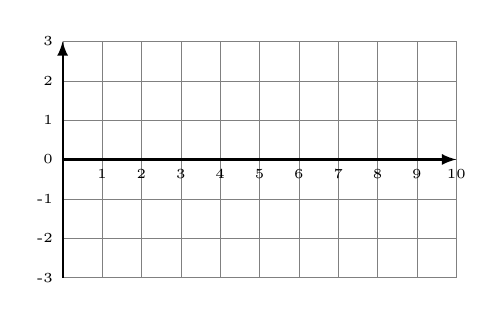
\begin{tikzpicture}[scale=0.5,domain=0:10]
        \draw[line width =0.03mm, gray] (0,-3) grid (10,3);
        \draw[thick, -latex] (0,0) -- (10,0);
        \draw[thick, -latex] (0,-3) -- (0,3);
        \foreach \x in {1,...,10} {
            \node[below] at (\x,0) {\tiny\x};
        }
        \foreach \y in {-3,-2,...,3} {
            \node[left] at (0,\y) {\tiny\y};
        }
        \foreach \n in {0,1,...,10} {
            \point{{\n}}{{-1*\n/3+2}}
        }
    \end{tikzpicture}
\end{center}

\question[2] Placer sur le graphique ci-dessous les dix termes : \vspace{-0.3cm}
$$u_0 = -1 ~~~~~~ u_1 = 2 ~~~~~~ u_2 = -2 ~~~~~~ u_3 = -2 ~~~~~~ u_4 = 3 ~~~~~~ u_5 = 0 ~~~~~~ u_6 = 1 ~~~~~~ u_7 = 2 ~~~~~~ u_8 = 3 ~~~~~~ u_9 = -3$$
    
\begin{center}
    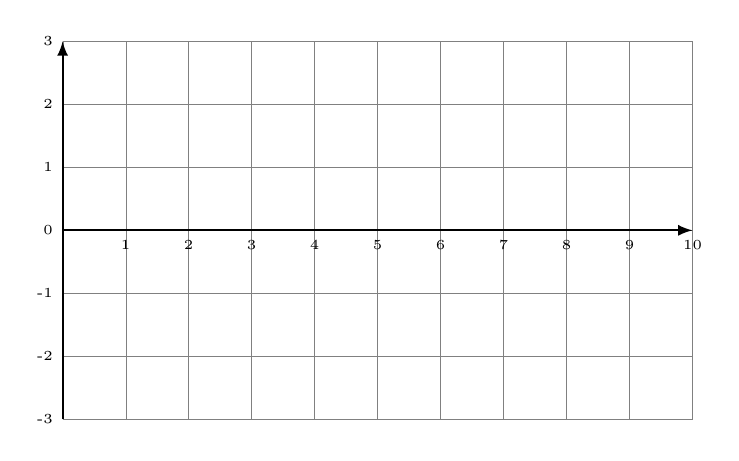
\begin{tikzpicture}[scale=0.8,domain=0:10]
        \draw[line width =0.03mm, gray] (0,-3) grid (10,3);
        \draw[thick, -latex] (0,0) -- (10,0);
        \draw[thick, -latex] (0,-3) -- (0,3);
        \foreach \x in {1,...,10} {
            \node[below] at (\x,0) {\tiny\x};
        }
        \foreach \y in {-3,-2,...,3} {
            \node[left] at (0,\y) {\tiny\y};
        }
    \end{tikzpicture}
\end{center}

\question[4]
\begin{parts}
    \part Soit la suite $(u_n)$ définie par $u_n = n^2 + 1$. Déterminer le signe de $u_{n+1} - u_n$.
    \part Soit la suite $(v_n)$ définie par $v_n = -2n+1$. Déterminer le signe de $v_{n+1} - v_n$.
\end{parts}

\end{questions}
\end{document}